\documentclass[a4paper, 12pt]{article}%тип документа

%отступы
\usepackage[left=2cm,right=2cm,top=2cm,bottom=3cm,bindingoffset=0cm]{geometry}

%Русский язык
\usepackage[T2A]{fontenc} %кодировка
\usepackage[utf8]{inputenc} %кодировка исходного кода
\usepackage[english,russian]{babel} %локализация и переносы

%Вставка картинок
\usepackage{graphicx}
\graphicspath{{pictures/}}
\DeclareGraphicsExtensions{.pdf,.png,.jpg}

%Графики
\usepackage{pgfplots}
\pgfplotsset{compat=1.9}

%Математика
\usepackage{amsmath, amsfonts, amssymb, amsthm, mathtools}

%Таблицы
\usepackage{longtable}


\begin{document}
	\begin{titlepage}
		\begin{center}
			\textsc{Федеральное государственное автономное образовательное учреждение высшего образования«Московский физико-технический институт (национальный исследовательский университет)»\\[5mm]
			}
			
			\vfill
			
			\textbf{Отчет по лабораторной работе 1.3.1-1.3.2\\[3mm]
				Определение модуля Юнга на основе исследования деформаций растяжения и определение модуля сдвига при помощи крутильных колебаний.
				\\[50mm]
			}
		\end{center}
		
		\hfill
		\begin{minipage}{.5\textwidth}
		Выполнил студент:\\[2mm] 
			Сериков Василий Романович\\[2mm] 
			группа: Б03-102\\[5mm]
			
		\end{minipage}
		\vfill
		\begin{center}
			Москва, 2021 г.
		\end{center}
\end{titlepage}
	
	\newpage
	\textbf{Цель работы:} экспериментально получить зависимость между напряжением и деформацией (закон Гука) для одноосного растяжения; по результатам измерений вычислить модуль Юнга. Измерение углов закручивания в зависимости от приложенного момента сил, расчет модулей кручения и сдвига для проволоки по измерениям периодов крутильных колебаний подвешенного на ней маятника. \\\\
	\textbf{В работе используется:} Прибор Лермантова, проволока из исследуемого материала, зрительная трубка со шкалой, набор грузов, микрометр, рулетка, линейка, грузы, штангенциркуль.\\\\
	\textbf{Теория:} В первой части работы производят растяжение проволоки, это соответствует случаю одноосного напряженного состояния. Для определения модуля Юнга используется прибор Лермантова (рис1). Удлинение проволоки можно измерить по углу поворота зеркальца.\\
	Во второй части работы вращение стержня с закрепленным на нем грузами (рис.2) вокруг вертикальной оси происходит под действием упругого момента, возникающего в проволоке.\\
	Модуль кручения: $f=\frac{\pi R^4G}{2l}$, где G-модуль сдвига
	\begin{figure}[h]
		\center{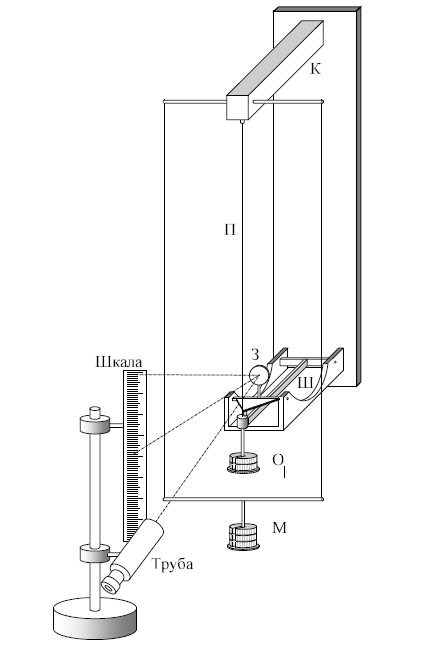
\includegraphics[scale=0.8]{jpej.png}}
	\end{figure}
	\center{\textbf{рис.1 }}
	\begin{figure}[h]
		\center{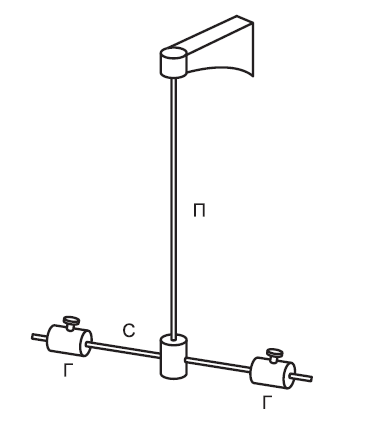
\includegraphics [scale=0.9]{Снимок экрана (380).png}}
	\end{figure}
	
	\newpage
	\center{\textbf{рис.2 }}
	\center{\textbf{Определение модуля Юнга по измерениям растяжения проволоки }}
	
	\begin{enumerate}
		\textbf{Ход работы}
		\item Диаметр проволоки - $d = (0,51 \pm 0,01) \text{мм}$.
		\item Вычисляем площадь поперечного сечения проволоки
		\[S =\dfrac{ \pi (\overline{d})^2}{4} = 0,204 \text{ мм}^2\]
		\[\sigma_S = S\sqrt{4\left( \dfrac{\sigma_d}{d}\right) ^2} = 0,007 \text{ мм}^2\]
		\[S = (0,204\pm0,007) \text{ мм}^2\]
		\item Измеряем длину проволоки $l = (173,0 \pm 0,1)\text{ см}$
		\item Направляем зрительную трубу на зеркальце так, чтобы мы четко видели шкалу, тогда свет от шкалы будет падать перпендикулярно шкале на зеркало, поэтому
		\[\Delta l =\dfrac{\Delta nr}{2h}\]
		\[ \sigma_{\Delta l} = \Delta l\sqrt{\left( \dfrac{\sigma_{n}}{n}\right)^2 + \left(\dfrac{\sigma_d}{d}\right)^2+\left(\dfrac{\sigma_h}{h}\right)^2} \]
		где $r = (20\pm 1)$ мм - расстояние от зеркала до проволоки, разница показаний шкалы - $n$, расстояние от шкалы до проволоки - $h = (134,3\pm0,1)\text{ см}$.
		\item Исходя из того, что $\sigma_{\text{предел}} = 900 \text{ Н}/\text{мм}^2$ получаем, что предельный вес, который можно повесить, чтобы не выйти за пределы $P_{\text{предел}} = 0,3 \sigma_{\text{предел}} S \approx 54 H$. 
		\item Снимем зависимость удлинения проволоки от массы грузов при увеличении и уменьшении нагрузки 3 раза (табл.1). 
		\item Построим график зависимости удлинения проволоки от нагрузки. Найдем уравнение получившийся прямой по МНК (график 1). По наклону прямой определим жесткость проволоки, а по ней - модуль Юнга. По МНК посчитаем погрешность значения k. (табл.2).
		
		\item По найденной графически жесткости проволоки найдем модуль Юнга по формуле
		\[E = \dfrac{Pl_0}{\Delta l S}\]
		\[\sigma_E = E\sqrt{\left( \dfrac{\sigma_{m}}{m} \right)^2 +\left( \dfrac{\sigma_{\Delta l}}{\Delta l} \right)^2+ \left( \dfrac{\sigma_{S}}{S} \right)^2 + \left( \dfrac{\sigma_{l_0}}{l_0} \right)^2 }\]
	\end{enumerate}
	\begin{figure}[h]
		\center{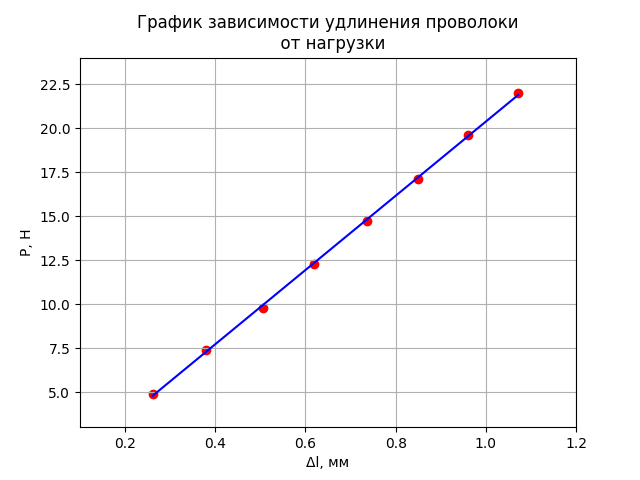
\includegraphics[scale=0.7]{first3.png}}
		\center {График 1}
	\end{figure}
\begin{longtable}{|c|c|c|c|c|c|c|c|c|c|}
				\hline
				P, Н & 2,45 &4,9 &7,4&9,8 &12,3 &14,7 &17,2 &19,6 &22,0 \\
				\hline
				$\Delta l$, мм&0,13 &0,26&	0,38&	0,51&	0,62&	0,74&	0,85& 0,96&	1.07
				\\ 
				\hline
				$\sigma_{\Delta l}$&0,01&	0,02&	0,02&	0,03&	0,03&	0,04&	0,04&	0,05&	0,05
				\\
				\hline
				\hline
				P, Н   &22,0&19,6  &17,2  &14,7&12,3&9,8&7,4 &4,9 &2,45\\
				\hline
				$\Delta l$, мм &1.07 &0,96 &0,85 &0,74 &0,62 &0,51 &0,38 &0,26 &0,13\\
				\hline
				$\sigma_{\Delta l}$&	0,05&	0,05&	0,04&	0,04&	0,03&	0,03&	0,02&	0,02&0,01 \\
				\hline
				\hline
				P, Н & 2,45 &4,9 &7,4&9,8 &12,3 &14,7 &17,2 &19,6 &22,0 \\
				\hline
				$\Delta l$, мм&0,13 &0,26&	0,37&	0,50&	0,62&	0,73&	0,84& 0,96&	1.07
				\\ 
				\hline
				$\sigma_{\Delta l}$&0,01&	0,02&	0,02&	0,03&	0,03&	0,04&	0,04&	0,05&	0,05
				\\
				\hline
				\hline
				P, Н   &22,0&19,6  &17,2  &14,7&12,3&9,8&7,4 &4,9 &2,45\\
				\hline
				$\Delta l$, мм&1.07 &0,96 &0,85 &0,74 &0,62 &0,51 &0,38 &0,26 &0,13\\
				\hline
				$\sigma_{\Delta l}$&	0,05&	0,05&	0,04&	0,04&	0,03&	0,03&	0,02&	0,02&0,01 \\
				\hline
				\hline
				P, Н & 2,45 &4,9 &7,4&9,8 &12,3 &14,7 &17,2 &19,6 &22,0 \\
				\hline
				$\Delta l$, мм&0,13 &0,26&	0,37&	0,50&	0,62&	0,73&	0,84& 0,96&	1.07
				\\ 
				\hline
				$\sigma_{\Delta l}$&0,01&	0,02&	0,02&	0,03&	0,03&	0,04&	0,04&	0,05&	0,05
				\\
				\hline
				\hline
				P, Н   &22,0&19,6  &17,2  &14,7&12,3&9,8&7,4 &4,9 &2,45\\
				\hline
				$\Delta l$, мм&1.07 &0,96 &0,85 &0,74 &0,62 &0,51 &0,38 &0,26 &0,13\\
				\hline
				$\sigma_{\Delta l}$&	0,05&	0,05&	0,04&	0,04&	0,03&	0,03&	0,02&	0,02&0,01\\
				\hline
				\caption{Зависимость удлинения проволоки от нагрузки.}
			\end{longtable}	
		
	\begin{longtable}{|c|c|c|}
				\hline
				&Значение&$\sigma$\\
				\hline
				k&$20, 9*10^3$ H/м&$0,5*10^3$ H/м\\
				\hline
				E&$13,4*10^{10}$ Па&$ 0,7*10^{10}$ Па\\
				\hline
				\caption{Значения k и E}
				\end{longtable}	
		
	\center{\textbf{Определение модуля модуля сдвига при помощи крутильных колебаний}}
	\begin{enumerate}
		\item Измеряем длину проволоки $l = (171,0 \pm 0,1)\text{ см}$
		\item Диаметр проволоки - $d = (1,56\pm 0,01) \text{мм}$.
		\item Измерим время  $ t_{1}$ 10 колебаний $: t_{1}=(19,2\pm 0,3)\text{с}$.
		\item Уменьшив амплитуду вдвое, измерим время $t_{2}$ 10 колебаний $: t_{2}=(19,1\pm0,3)\text{с}$.
		\item Таким образом получаем: $t_{1}\approx  t_{2} \text{ в пределах погрешности}$. Также мы установили, что после 10 колебаний амплитуда уменьшается менее чем в 2 раза.
		\item Установим грузы на стержне на одинаковом расстоянии l от оси проволоки до центра масс каждого грузика и измерим период колебаний T для 7 различных значений l дважды (чтобы исключить возможность промаха), данные занесем в таблицу 3 ($\sigma_l$=0,1 см, $\sigma_T$= 0.03 с). Величину модуля кручения найдем из наклона прямой линии, проведенной по экспериментальным точкам, отложенным в координатах $l^2, T^2$ (график 2). Период колебаний можно рассчитать по формуле	$$T^2=\frac{(2 \pi)^2}{f} I_0 + \frac{(2 \pi)^2}{f} 2m \cdot l^2$$, где $I_0$ - момент инерции системы без грузов, $l$ - длина проволоки, $T$ - период колебаний при заданной длине $l$, $m$ - масса одного груза. Тогда коэффициент наклона прямой будет равен $k=\frac{(2 \pi)^2}{f} 2m$, отсюда $f=\frac{(2 \pi)^2}{k} 2m$, m = 205,1г. По МНК посчитаем значение k и b и их погрешности. $T^2=kl^2+b$
		\item По найденному модулю кручения с помощью формулы $f=\frac{\pi d^4G}{32l}$ получим модуль сдвига G, оценим погрешности измерения, данные занесем в таблицу 4.\\
		$f=\frac{4\pi^22ml^2}{T^2-b} \implies \sigma_{f}= \sqrt{(\frac{\partial f}{\partial m}\sigma_m)^2 + (\frac{\partial f}{\partial T}\sigma_{T})^2 + (\frac{\partial f}{\partial l}\sigma_{l})^2}$\\
		
		$\sigma_G = G\sqrt{\left( \dfrac{\sigma_{f}}{f} \right)^2 +\left( \dfrac{\sigma_{ l}}{l} \right)^2+ 16\left( \dfrac{\sigma_{d}}{d}\right)^2 }$
		
		
	\begin{longtable}{|c|c|c|c|c|c|c|c|c|c|c|c|c|c|c|}
					\hline
					№ & 1 &2 &3 &4 &5 &6 &7 &8 &9 &10 &11 &12 &13 &14 \\
					\hline
					T, c &1,91 &1,92 &2,04 &2,04 &2,25 &2,23 &2,47 &2,43 &2,66 &2,65 &2,92 &2,90 &3,13 &3,14
					\\ 
					\hline
					l, см &4,5 &4,5 &5,5 &5,5 &6,5 &6,5 &7,5 &7,5 &8,5 &8,5 &9,5 &9,5 &10,5 &10,5
					\\
					\hline
					
					\caption{Зависимость периода от расстояния от проволоки до центра масс грузика}
				\end{longtable}	
			
	\begin{longtable}{|c|c|c|}
		\hline
		&Значение&$\sigma$\\
		\hline
		k&$418,5$$\text{ c}^2/\text{м}^2$&0,5 $\text{ c}^2/\text{м}^2$\\
		\hline
		b& $3,18\text{ c}^2$& 0,08 $\text{c}^2$ \\
		\hline
		f&$56,51\text{ Н}\cdot \text{мм/рад}$ &$ 0,06\text{ Н}\cdot \text{мм/рад}$\\
		\hline
		G&$83,8$ ГПа&$ 0,5$ ГПа \\
		\hline
		
		\caption{Значения k,b, f, G}
	\end{longtable}	
		
		\begin{figure}[h]
			\center{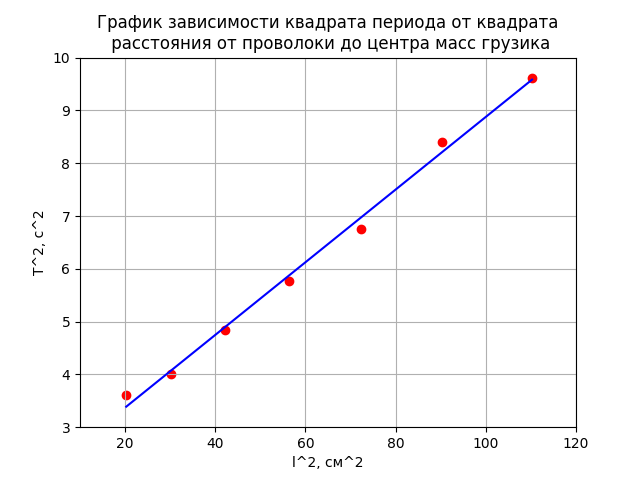
\includegraphics [scale=0.7]{first2.png} \center график 2}
		\end{figure}
		
		
		\item \textbf{Вывод:} Таким образом, сделав две работы по изучению модуля Юнга и модуля сдвига проволоки, мы установили что материал, из которого изготовлены проволоки - это низко углеродистая сталь.
	\end{enumerate}
\end{document}